% Options for packages loaded elsewhere
\PassOptionsToPackage{unicode}{hyperref}
\PassOptionsToPackage{hyphens}{url}
%
\documentclass[
]{article}
\usepackage{amsmath,amssymb}
\usepackage{lmodern}
\usepackage{ifxetex,ifluatex}
\ifnum 0\ifxetex 1\fi\ifluatex 1\fi=0 % if pdftex
  \usepackage[T1]{fontenc}
  \usepackage[utf8]{inputenc}
  \usepackage{textcomp} % provide euro and other symbols
\else % if luatex or xetex
  \usepackage{unicode-math}
  \defaultfontfeatures{Scale=MatchLowercase}
  \defaultfontfeatures[\rmfamily]{Ligatures=TeX,Scale=1}
\fi
% Use upquote if available, for straight quotes in verbatim environments
\IfFileExists{upquote.sty}{\usepackage{upquote}}{}
\IfFileExists{microtype.sty}{% use microtype if available
  \usepackage[]{microtype}
  \UseMicrotypeSet[protrusion]{basicmath} % disable protrusion for tt fonts
}{}
\makeatletter
\@ifundefined{KOMAClassName}{% if non-KOMA class
  \IfFileExists{parskip.sty}{%
    \usepackage{parskip}
  }{% else
    \setlength{\parindent}{0pt}
    \setlength{\parskip}{6pt plus 2pt minus 1pt}}
}{% if KOMA class
  \KOMAoptions{parskip=half}}
\makeatother
\usepackage{xcolor}
\IfFileExists{xurl.sty}{\usepackage{xurl}}{} % add URL line breaks if available
\IfFileExists{bookmark.sty}{\usepackage{bookmark}}{\usepackage{hyperref}}
\hypersetup{
  pdftitle={Lab 03 - Health care spending and coverage in the US},
  pdfauthor={Emma Gardecki},
  hidelinks,
  pdfcreator={LaTeX via pandoc}}
\urlstyle{same} % disable monospaced font for URLs
\usepackage[margin=1in]{geometry}
\usepackage{color}
\usepackage{fancyvrb}
\newcommand{\VerbBar}{|}
\newcommand{\VERB}{\Verb[commandchars=\\\{\}]}
\DefineVerbatimEnvironment{Highlighting}{Verbatim}{commandchars=\\\{\}}
% Add ',fontsize=\small' for more characters per line
\usepackage{framed}
\definecolor{shadecolor}{RGB}{248,248,248}
\newenvironment{Shaded}{\begin{snugshade}}{\end{snugshade}}
\newcommand{\AlertTok}[1]{\textcolor[rgb]{0.94,0.16,0.16}{#1}}
\newcommand{\AnnotationTok}[1]{\textcolor[rgb]{0.56,0.35,0.01}{\textbf{\textit{#1}}}}
\newcommand{\AttributeTok}[1]{\textcolor[rgb]{0.77,0.63,0.00}{#1}}
\newcommand{\BaseNTok}[1]{\textcolor[rgb]{0.00,0.00,0.81}{#1}}
\newcommand{\BuiltInTok}[1]{#1}
\newcommand{\CharTok}[1]{\textcolor[rgb]{0.31,0.60,0.02}{#1}}
\newcommand{\CommentTok}[1]{\textcolor[rgb]{0.56,0.35,0.01}{\textit{#1}}}
\newcommand{\CommentVarTok}[1]{\textcolor[rgb]{0.56,0.35,0.01}{\textbf{\textit{#1}}}}
\newcommand{\ConstantTok}[1]{\textcolor[rgb]{0.00,0.00,0.00}{#1}}
\newcommand{\ControlFlowTok}[1]{\textcolor[rgb]{0.13,0.29,0.53}{\textbf{#1}}}
\newcommand{\DataTypeTok}[1]{\textcolor[rgb]{0.13,0.29,0.53}{#1}}
\newcommand{\DecValTok}[1]{\textcolor[rgb]{0.00,0.00,0.81}{#1}}
\newcommand{\DocumentationTok}[1]{\textcolor[rgb]{0.56,0.35,0.01}{\textbf{\textit{#1}}}}
\newcommand{\ErrorTok}[1]{\textcolor[rgb]{0.64,0.00,0.00}{\textbf{#1}}}
\newcommand{\ExtensionTok}[1]{#1}
\newcommand{\FloatTok}[1]{\textcolor[rgb]{0.00,0.00,0.81}{#1}}
\newcommand{\FunctionTok}[1]{\textcolor[rgb]{0.00,0.00,0.00}{#1}}
\newcommand{\ImportTok}[1]{#1}
\newcommand{\InformationTok}[1]{\textcolor[rgb]{0.56,0.35,0.01}{\textbf{\textit{#1}}}}
\newcommand{\KeywordTok}[1]{\textcolor[rgb]{0.13,0.29,0.53}{\textbf{#1}}}
\newcommand{\NormalTok}[1]{#1}
\newcommand{\OperatorTok}[1]{\textcolor[rgb]{0.81,0.36,0.00}{\textbf{#1}}}
\newcommand{\OtherTok}[1]{\textcolor[rgb]{0.56,0.35,0.01}{#1}}
\newcommand{\PreprocessorTok}[1]{\textcolor[rgb]{0.56,0.35,0.01}{\textit{#1}}}
\newcommand{\RegionMarkerTok}[1]{#1}
\newcommand{\SpecialCharTok}[1]{\textcolor[rgb]{0.00,0.00,0.00}{#1}}
\newcommand{\SpecialStringTok}[1]{\textcolor[rgb]{0.31,0.60,0.02}{#1}}
\newcommand{\StringTok}[1]{\textcolor[rgb]{0.31,0.60,0.02}{#1}}
\newcommand{\VariableTok}[1]{\textcolor[rgb]{0.00,0.00,0.00}{#1}}
\newcommand{\VerbatimStringTok}[1]{\textcolor[rgb]{0.31,0.60,0.02}{#1}}
\newcommand{\WarningTok}[1]{\textcolor[rgb]{0.56,0.35,0.01}{\textbf{\textit{#1}}}}
\usepackage{graphicx}
\makeatletter
\def\maxwidth{\ifdim\Gin@nat@width>\linewidth\linewidth\else\Gin@nat@width\fi}
\def\maxheight{\ifdim\Gin@nat@height>\textheight\textheight\else\Gin@nat@height\fi}
\makeatother
% Scale images if necessary, so that they will not overflow the page
% margins by default, and it is still possible to overwrite the defaults
% using explicit options in \includegraphics[width, height, ...]{}
\setkeys{Gin}{width=\maxwidth,height=\maxheight,keepaspectratio}
% Set default figure placement to htbp
\makeatletter
\def\fps@figure{htbp}
\makeatother
\setlength{\emergencystretch}{3em} % prevent overfull lines
\providecommand{\tightlist}{%
  \setlength{\itemsep}{0pt}\setlength{\parskip}{0pt}}
\setcounter{secnumdepth}{-\maxdimen} % remove section numbering
\ifluatex
  \usepackage{selnolig}  % disable illegal ligatures
\fi

\title{Lab 03 - Health care spending and coverage in the US}
\usepackage{etoolbox}
\makeatletter
\providecommand{\subtitle}[1]{% add subtitle to \maketitle
  \apptocmd{\@title}{\par {\large #1 \par}}{}{}
}
\makeatother
\subtitle{Data Wrangling + Tidy Data}
\author{Emma Gardecki}
\date{2021-03-04}

\begin{document}
\maketitle

{
\setcounter{tocdepth}{2}
\tableofcontents
}
These exercises are designed to give you practice wrangling and tidying
data, both from a \emph{processes} perspective (what needs to be done to
the data before I can run my fancy analysis and/or make my cool
visualization?) and an \emph{R implementation} perspective (how do I
implement those steps specifically in R?).

\hypertarget{packages}{%
\section{Packages}\label{packages}}

In this lab we will work with the \texttt{tidyverse}, \texttt{datasets},
and \texttt{janitor} packages. The \texttt{datasets} package contains a
dataset \texttt{state} with information on each state such as region.

We start by loading the packages.

\begin{Shaded}
\begin{Highlighting}[]
\FunctionTok{library}\NormalTok{(tidyverse)}
\FunctionTok{library}\NormalTok{(datasets)}
\FunctionTok{library}\NormalTok{(janitor)}
\end{Highlighting}
\end{Shaded}

\hypertarget{exploring-health-expenditure-using-state-level-data}{%
\section{Exploring Health Expenditure using State-level
data}\label{exploring-health-expenditure-using-state-level-data}}

This case study is based on an open case study from the OCS project (Kuo
et al.~2019).

Health policy in the United States is complicated, and several forms of
health care coverage exist, including both federal government-led health
care policy, and private insurance company. Before making any inference
about the relationship between health condition and health policy, it is
important for us to have a general idea about health care economics in
the United States. Thus, we are interested in getting a sense of the
health expenditure, including health care coverage and health care
spending, across the United States.

Motivating questions:

\begin{itemize}
\tightlist
\item
  Is there a relationship between health care coverage and health care
  spending in the United States?
\item
  How does the spending distribution change across geographic regions in
  the United States?
\item
  Does the relationship between health care coverage and health care
  spending in the United States change from 2013 to 2014?
\end{itemize}

\hypertarget{the-data}{%
\section{The Data}\label{the-data}}

Data for this lab come from Henry J Kaiser Family Foundation (KFF).

\begin{itemize}
\tightlist
\item
  Health Insurance Coverage of the Total
  Population{[}\url{https://www.kff.org/other/state-indicator/total-population/}{]}

  \begin{itemize}
  \tightlist
  \item
    Includes years 2013-2016
  \end{itemize}
\item
  Health Care Expenditures by State of Residence (in
  millions){[}\url{https://www.kff.org/other/state-indicator/health-care-expenditures-by-state-of-residence-in-millions/?currentTimeframe=0\&sortModel=\%7B\%22colId\%22:\%22Location\%22,\%22sort\%22:\%22asc\%22\%7D}{]}

  \begin{itemize}
  \tightlist
  \item
    Includes years 1991-2014
  \end{itemize}
\end{itemize}

First, let's read in the files containing the healthcare coverage and
healthcare spending data.

\emph{Getting an error trying to read in the data? Watch the video
``Lab03-filepaths'' (posted on Moodle) for help troubleshooting.}

\begin{Shaded}
\begin{Highlighting}[]
\NormalTok{coverage }\OtherTok{\textless{}{-}} \FunctionTok{read\_csv}\NormalTok{(}\StringTok{"C:/Users/Lorraine/Dropbox/Data Science/Data{-}Science/data/healthcare\_coverage.txt"}\NormalTok{)}
\NormalTok{spending }\OtherTok{\textless{}{-}} \FunctionTok{read\_csv}\NormalTok{(}\StringTok{"C:/Users/Lorraine/Dropbox/Data Science/Data{-}Science/data/healthcare\_spending.txt"}\NormalTok{)}
\end{Highlighting}
\end{Shaded}

\begin{Shaded}
\begin{Highlighting}[]
\CommentTok{\#coverage \textless{}{-} read\_csv("/Users/emmagardecki/Documents/junior yr/stat231/stat231g/data/healthcare\_coverage.txt")}
\CommentTok{\#spending \textless{}{-} read\_csv("/Users/emmagardecki/Documents/junior yr/stat231/stat231g/data/healthcare\_spending.txt")}
\end{Highlighting}
\end{Shaded}

\begin{Shaded}
\begin{Highlighting}[]
\NormalTok{coverage1 }\OtherTok{\textless{}{-}} \FunctionTok{mutate}\NormalTok{( coverage, }\AttributeTok{.before =} \StringTok{"Location"}\NormalTok{, }\AttributeTok{num =} \FunctionTok{row\_number}\NormalTok{(  }\FunctionTok{c}\NormalTok{( }\DecValTok{1}\SpecialCharTok{:}\DecValTok{52}\NormalTok{ ) )) }
\NormalTok{spending1 }\OtherTok{\textless{}{-}} \FunctionTok{mutate}\NormalTok{( spending, }\AttributeTok{.before =} \StringTok{"Location"}\NormalTok{, }\AttributeTok{num =} \FunctionTok{row\_number}\NormalTok{( }\FunctionTok{c}\NormalTok{( }\DecValTok{1}\SpecialCharTok{:}\DecValTok{52}\NormalTok{ )))}
\end{Highlighting}
\end{Shaded}

Since our goal is to get sense of the health expenditure, including
health care coverage and health care spending, across states, it would
be nice add some information about each state. Namely, the state
abbreviation and state region (i.e.~north, south, etc).

For this we use the \texttt{state} dataset in the \texttt{datasets} R
package. Since we already loaded that package, we can refer directly to
the \texttt{state} dataset even though we don't see it in our
Environment pane in the upper right corner. However, I like to be able
to see any objects I'm working with in my Environment, so run the
following code:

\begin{Shaded}
\begin{Highlighting}[]
\CommentTok{\# state objects should appear in your Environment pane}
\FunctionTok{data}\NormalTok{(state) }

\CommentTok{\# creates a data frame with state info}
\NormalTok{state\_info }\OtherTok{\textless{}{-}} \FunctionTok{data.frame}\NormalTok{(}\AttributeTok{Location =}\NormalTok{ state.name, }\AttributeTok{Abbrev =}\NormalTok{ state.abb, }\AttributeTok{Region =}\NormalTok{ state.region)}
\end{Highlighting}
\end{Shaded}

\hypertarget{warm-up}{%
\section{Warm-up}\label{warm-up}}

Get acquainted with the \texttt{spending} and \texttt{coverage}
datasets. What years are covered in the \texttt{spending} dataset? What
years are covered in the \texttt{coverage} dataset? (Yes, the answers to
these questions are above, but how can you confirm this in the
datasets?)

If we're interested in the relationship between spending and coverage,
we'll only be able to use observations that have information on both.
That is, we won't be using data from years for which we only have
spending information or only have coverage information. Remove any
variables we won't be using from \texttt{spending} and
\texttt{coverage}. (Hint: the \texttt{starts\_with} function could help
with efficiency here:
\url{https://tidyselect.r-lib.org/reference/starts_with.html})

\begin{quote}
RESPONSE: The spending dataset covers the years 1991 to 2014, while the
coverage dataset covers the years 2013 to 2016. Therefore, the
overlapping data only includes the years 2013 and 2014.
\end{quote}

\begin{Shaded}
\begin{Highlighting}[]
\CommentTok{\#creates combined dataframe and cleans it up to feature only location, and yrs 2013, 2014}
\NormalTok{spend\_cov }\OtherTok{\textless{}{-}} \FunctionTok{merge}\NormalTok{( spending1, coverage1, }\AttributeTok{by =} \StringTok{"num"}\NormalTok{)}
\NormalTok{spend\_cov }\OtherTok{\textless{}{-}}\NormalTok{ spend\_cov }\SpecialCharTok{\%\textgreater{}\%}
  \FunctionTok{select}\NormalTok{( }\FunctionTok{starts\_with}\NormalTok{( }\FunctionTok{c}\NormalTok{( }\StringTok{"Location"}\NormalTok{,}\StringTok{"2013"}\NormalTok{, }\StringTok{"2014"}\NormalTok{))) }
\NormalTok{spend\_cov}\SpecialCharTok{$}\NormalTok{Location.x}\OtherTok{\textless{}{-}} \ConstantTok{NULL}
\NormalTok{spend\_cov }\OtherTok{\textless{}{-}} \FunctionTok{rename}\NormalTok{( spend\_cov, }\StringTok{"Location"} \OtherTok{=}\NormalTok{ Location.y )}
\end{Highlighting}
\end{Shaded}

Note that there are observations both for the US as a whole and DC.
Remove these observations from both datasets.

\begin{Shaded}
\begin{Highlighting}[]
\NormalTok{spend\_cov }\OtherTok{\textless{}{-}}\NormalTok{ spend\_cov[ }\SpecialCharTok{{-}}\FunctionTok{c}\NormalTok{( }\DecValTok{1}\NormalTok{, }\DecValTok{10}\NormalTok{ ), ] }
\end{Highlighting}
\end{Shaded}

\emph{This is a good place to pause, commit changes with the commit
message ``Added answer for Warm-up'', and push.}

\hypertarget{health-care-spending-and-coverage}{%
\section{Health care spending and
coverage}\label{health-care-spending-and-coverage}}

\hypertarget{q1.-is-there-a-relationship-between-healthcare-coverage-and-healthcare-spending-in-the-united-states}{%
\subsection{Q1. Is there a relationship between healthcare coverage and
healthcare spending in the United
States?}\label{q1.-is-there-a-relationship-between-healthcare-coverage-and-healthcare-spending-in-the-united-states}}

Let's start by creating a scatterplot with log(spending) on the x-axis
and log(employer coverage) on the y-axis, with the points colored by
year. (Note that we'll use logs because both these variables are
right-skewed and have large outliers; feel free to check out their
histograms and/or look at the un-logged scatterplot if you'd like, as
well.) This is a simple enough scatterplot, but we'll need to do a bit
of data tidying before the data are in an appropriate format to create
the plot.

First, sketch the scatterplot (don't worry about the actual x-y
relationship, but be sure to identify the different variables that will
be needed to create the plot). What variables do you need in the dataset
in order to create the scatterplot in ggplot? What will each observation
(row) in the dataset represent?

\begin{quote}
RESPONSE: ggplot(spend\_cov, aes(log(total health spending),
log(employer))) + geom\_point(color = year).
\end{quote}

What are some of the steps that will need to be taken to get the data in
that form?

\begin{quote}
RESPONSE: We need to make year a variable and merge all of the matching
varibales together (aka 2013 and 2014 employer, etc.)
\end{quote}

\emph{When you're done with the above responses, check that you're on
the right track by viewing the video ``Lab03-q1-sketch'' (posted on
Moodle).}

Now implement those steps in R, tidying the dataset for plotting. After
the final step, use the \texttt{clean\_names()} function from the
\texttt{janitor} package to clean the variable names. Then, create the
scatterplot.

\emph{Having trouble trying to figure out how to implement your steps in
R? Get some hints from the video ``Lab03-q1-steps'' (posted on Moodle).
Be sure you give a sufficient effort on your own first; the struggle
helps you learn and remember!}

\begin{Shaded}
\begin{Highlighting}[]
\NormalTok{spend\_cov }\OtherTok{\textless{}{-}}\NormalTok{ spend\_cov }\SpecialCharTok{\%\textgreater{}\%}
  \FunctionTok{clean\_names}\NormalTok{()}

\CommentTok{\#separates spend\_cov dataset into 2013 and 2014 }
\NormalTok{spend\_cov2013 }\OtherTok{\textless{}{-}}\NormalTok{ spend\_cov }\SpecialCharTok{\%\textgreater{}\%}
  \FunctionTok{select}\NormalTok{( }\FunctionTok{starts\_with}\NormalTok{( }\FunctionTok{c}\NormalTok{( }\StringTok{"Location"}\NormalTok{,}\StringTok{"x2013"}\NormalTok{))) }

\NormalTok{spend\_cov2014 }\OtherTok{\textless{}{-}}\NormalTok{ spend\_cov }\SpecialCharTok{\%\textgreater{}\%}
  \FunctionTok{select}\NormalTok{( }\FunctionTok{starts\_with}\NormalTok{( }\FunctionTok{c}\NormalTok{( }\StringTok{"Location"}\NormalTok{, }\StringTok{"x2014"}\NormalTok{ )))}
\end{Highlighting}
\end{Shaded}

\begin{Shaded}
\begin{Highlighting}[]
\CommentTok{\#adds year column and cleans all the var names}
\NormalTok{spend\_cov2013}\SpecialCharTok{$}\NormalTok{year }\OtherTok{\textless{}{-}} \StringTok{"2013"}
\NormalTok{spend\_cov2013 }\OtherTok{\textless{}{-}} 
  \FunctionTok{rename}\NormalTok{( spend\_cov2013, }\FunctionTok{c}\NormalTok{(}\StringTok{"spending"} \OtherTok{=}\NormalTok{ x2013\_total\_health\_spending, }\StringTok{"employer"} \OtherTok{=}\NormalTok{ x2013\_employer, }\StringTok{"non\_group"} \OtherTok{=}\NormalTok{ x2013\_non\_group, }\StringTok{"medicaid"} \OtherTok{=}\NormalTok{ x2013\_medicaid, }\StringTok{"medicare"} \OtherTok{=}\NormalTok{ x2013\_medicare, }\StringTok{"other\_public"} \OtherTok{=}\NormalTok{ x2013\_other\_public, }\StringTok{"uninsured"} \OtherTok{=}\NormalTok{ x2013\_uninsured, }\StringTok{"total"} \OtherTok{=}\NormalTok{ x2013\_total))}

\NormalTok{spend\_cov2014}\SpecialCharTok{$}\NormalTok{year }\OtherTok{\textless{}{-}} \StringTok{"2014"}
\NormalTok{spend\_cov2014 }\OtherTok{\textless{}{-}} 
  \FunctionTok{rename}\NormalTok{( spend\_cov2014, }\FunctionTok{c}\NormalTok{(}\StringTok{"spending"} \OtherTok{=}\NormalTok{ x2014\_total\_health\_spending, }\StringTok{"employer"} \OtherTok{=}\NormalTok{ x2014\_employer, }\StringTok{"non\_group"} \OtherTok{=}\NormalTok{ x2014\_non\_group, }\StringTok{"medicaid"} \OtherTok{=}\NormalTok{ x2014\_medicaid, }\StringTok{"medicare"} \OtherTok{=}\NormalTok{ x2014\_medicare, }\StringTok{"other\_public"} \OtherTok{=}\NormalTok{ x2014\_other\_public, }\StringTok{"uninsured"} \OtherTok{=}\NormalTok{ x2014\_uninsured, }\StringTok{"total"} \OtherTok{=}\NormalTok{ x2014\_total))}

\CommentTok{\#merges datasets back together now with double the cases }
\NormalTok{spend\_cov2 }\OtherTok{\textless{}{-}} \FunctionTok{rbind}\NormalTok{( spend\_cov2013, spend\_cov2014)}
\end{Highlighting}
\end{Shaded}

\begin{Shaded}
\begin{Highlighting}[]
\FunctionTok{ggplot}\NormalTok{( spend\_cov2, }\FunctionTok{aes}\NormalTok{( }\FunctionTok{log}\NormalTok{(spending), }\FunctionTok{log}\NormalTok{(employer))) }\SpecialCharTok{+} \FunctionTok{geom\_point}\NormalTok{( }\FunctionTok{aes}\NormalTok{( }\AttributeTok{color =}\NormalTok{ year ))}
\end{Highlighting}
\end{Shaded}

\includegraphics{gardecki_lab03-wrangle-tidy_files/figure-latex/unnamed-chunk-11-1.pdf}

We see there is a strong relationship between log(spending) and
log(coverage) within each year. However, you might suspect that health
care coverage and spending is also strongly related to population size.
In the \texttt{coverage} dataset, the total type is not really a formal
type of health care coverage. It really represents just the total number
of people in the state. This is useful information. Next:

\begin{itemize}
\tightlist
\item
  rename that column to be \texttt{total\_pop} to be clear.
\item
  create a scatterplot of \texttt{total\_pop} (population size) versus
  employer coverage
\item
  create a scatterplot of \texttt{total\_pop} (population size) versus
  spending
\end{itemize}

What do you notice?

\begin{quote}
RESPONSE: In both scatterplots below there is still a strong positive
relationship. However, these plots are more densely populated near (0,
0) and feature wide gaps as the total population increases (and thus the
spending as well).
\end{quote}

\begin{Shaded}
\begin{Highlighting}[]
\NormalTok{ spend\_cov2 }\OtherTok{\textless{}{-}} \FunctionTok{rename}\NormalTok{( spend\_cov2, }\StringTok{"total\_pop"} \OtherTok{=}\NormalTok{ total)}

\FunctionTok{ggplot}\NormalTok{( spend\_cov2, }\FunctionTok{aes}\NormalTok{( total\_pop, employer)) }\SpecialCharTok{+} \FunctionTok{geom\_point}\NormalTok{( }\FunctionTok{aes}\NormalTok{( }\AttributeTok{color =}\NormalTok{ year))}
\end{Highlighting}
\end{Shaded}

\includegraphics{gardecki_lab03-wrangle-tidy_files/figure-latex/unnamed-chunk-12-1.pdf}

\begin{Shaded}
\begin{Highlighting}[]
\FunctionTok{ggplot}\NormalTok{( spend\_cov2, }\FunctionTok{aes}\NormalTok{( total\_pop, spending)) }\SpecialCharTok{+} \FunctionTok{geom\_point}\NormalTok{( }\FunctionTok{aes}\NormalTok{( }\AttributeTok{color =}\NormalTok{ year))}
\end{Highlighting}
\end{Shaded}

\includegraphics{gardecki_lab03-wrangle-tidy_files/figure-latex/unnamed-chunk-12-2.pdf}

Lastly, to account for total population, create a scatterplot of
spending per capita versus proportion with employer coverage. This time,
\emph{color by region} and \emph{facet by year}. The total spending
column is reported in millions (1e6). Therefore, to calculate
\texttt{spending\_capita} we will need to adjust for this scaling factor
to report it on the original scale (just dollars) and then divide by
\texttt{tot\_pop}. Based on this figure, write a brief paragraph
describing the relationship between health care spending and coverage in
the US.

\begin{quote}
RESPONSE:
\end{quote}

\emph{This is a good place to pause, commit changes with the commit
message ``Added answer for Q1'', and push.}

\hypertarget{which-us-states-spend-the-most-and-which-spend-the-least-on-health-care-how-does-the-spending-distribution-change-across-geographic-regions-in-the-united-states}{%
\subsection{Which US states spend the most and which spend the least on
health care? How does the spending distribution change across geographic
regions in the United
States?}\label{which-us-states-spend-the-most-and-which-spend-the-least-on-health-care-how-does-the-spending-distribution-change-across-geographic-regions-in-the-united-states}}

Which US states spent the most per capita on health care in 2013 and
2014?

\begin{quote}
RESPONSE:
\end{quote}

Which US states spent the least per capita on health care in 2013 and
2014?

\begin{quote}
RESPONSE:
\end{quote}

How does the spending distribution change across geographic region in
the US? Create an appropriate figure to visualize the distribution of
spending per capita on health care by region. Write one paragraph
summarizing a comparison of the distributions. (Note that you probably
will also want to generate summary statistics by region in order to
include specific values in your summary paragraph.)

\begin{quote}
RESPONSE:
\end{quote}

\emph{This is a good place to pause, commit changes with the commit
message ``Added answer for Q2'', and push.}

\hypertarget{does-the-relationship-between-healthcare-spending-and-the-proportion-of-uninsured-in-the-united-states-change-from-2013-to-2014}{%
\subsection{Does the relationship between healthcare spending and the
proportion of uninsured in the United States change from 2013 to
2014?}\label{does-the-relationship-between-healthcare-spending-and-the-proportion-of-uninsured-in-the-united-states-change-from-2013-to-2014}}

Re-create this plot for 2013:
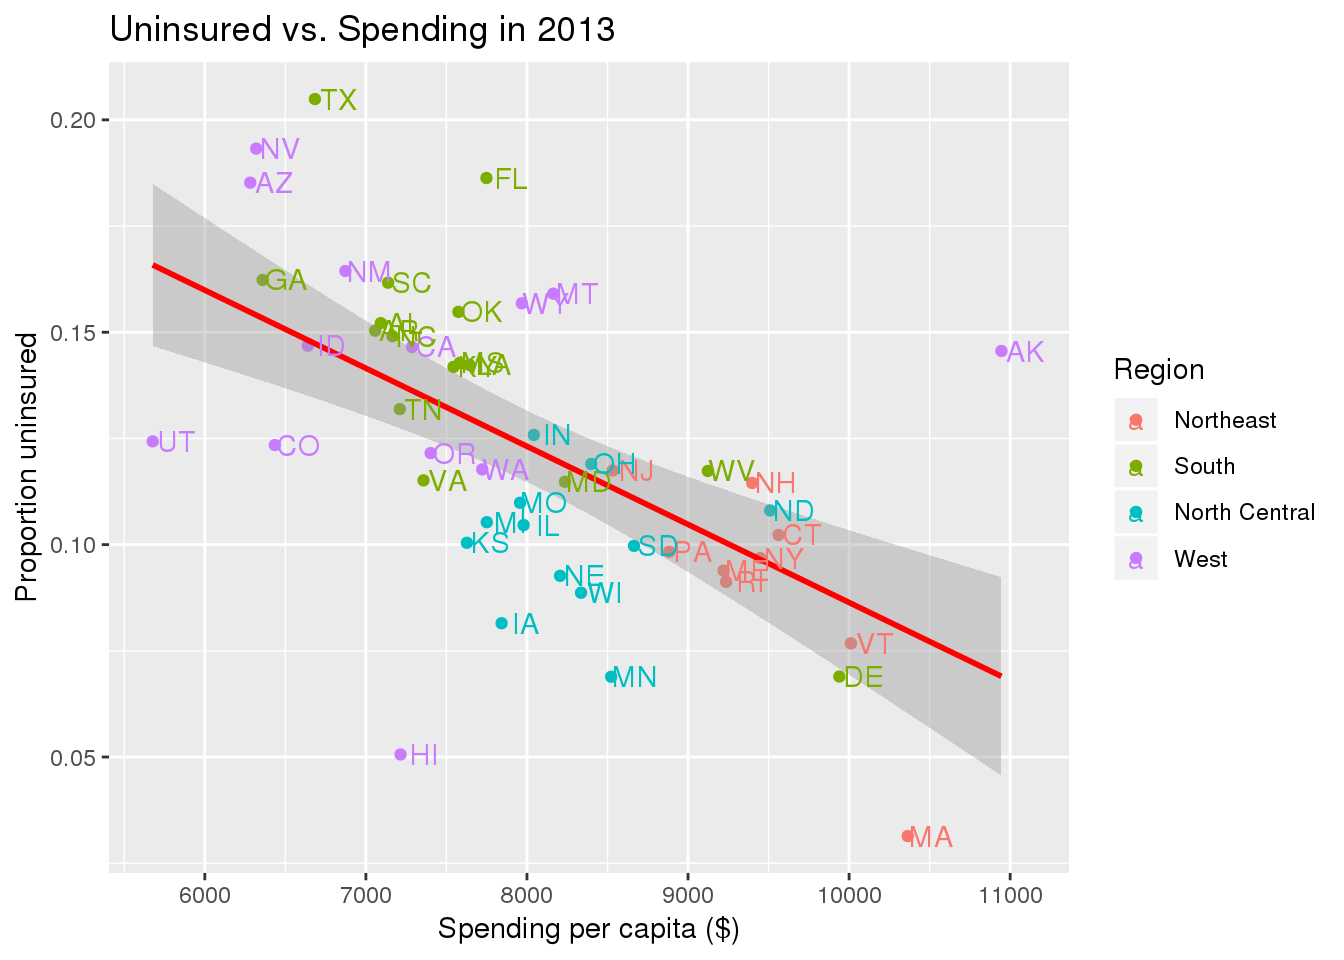
\includegraphics{images/uninsured_spending_2013.png}

(Hint: use \texttt{nudge\_x\ =\ 150} in the \texttt{geom\_text} layer.)

Next, create an analogous plot (separately) for 2014. Does the
relationship between health care spending and the proportion of
uninsured change from 2013 to 2014?

\begin{quote}
RESPONSE:
\end{quote}

Create the same plots, but instead of creating completely separate
figures for 2013 and 2014, create one figure that is facetted by year
(still colored by region).

Lastly, plot the points for both years on the same plot, this time
colored by year instead of region. Make sure to specify the
\texttt{group} aesthetic for year as well to get two lines.

Which of these three visualizations do you find most helpful for
comparing the relationship between 2013 and 2014? Why?

\begin{quote}
RESPONSE:
\end{quote}

\emph{This is a good place to pause, commit changes with the commit
message ``Added answer for Q3'', and push.}

\hypertarget{extra}{%
\subsection{Extra}\label{extra}}

Done early? Try to figure out how to make these additional updates to
the first figure from the last exercise to hone your plotting skills:

\begin{itemize}
\tightlist
\item
  remove the ``a'' on the points in the legend
\item
  change the background to be all white
\item
  make the numbers on the x-axis larger
\item
  change the font of the text on the y-axis
\end{itemize}

\hypertarget{references}{%
\section{References}\label{references}}

Kuo, Pei-Lun and Jager, Leah and Taub, Margaret and Hicks, Stephanie.
(2019, February 14). opencasestudies/ocs-healthexpenditure: Exploring
Health Expenditure using State-level data in the United States (Version
v1.0.0). Zenodo. \url{http://doi.org/10.5281/zenodo.2565307}

\end{document}
